\documentclass[aspectratio=169, 10pt]{beamer}

% ============================================================
% Lecture 2: DiD — The Good, the Bad, and the Ugly
% PhD programme: Economics, Management and Methods for the
% Sustainable Transition — University of Ferrara, 6 May 2026
% Author: Francesco Rentocchini
% Source material: Cunningham CI-2 (2024), Advanced-DiD (Roth),
%   Goodman-Bacon (2021), Callaway & Sant'Anna (2021),
%   Sun & Abraham (2021), Rambachan & Roth (2023)
% ============================================================

\usetheme{default}
% ============================================================
% preamble.tex — fit_phd_lectures
% Adapted from Scott Cunningham's Causal Inference Mixtape Sessions
% Compatible with pdflatex
% ============================================================

% --- Colors — JRC / European Commission identity ------------
\usepackage{xcolor}

% EC / JRC brand palette — softer pastel-leaning blue
\definecolor{ecblue}{HTML}{2E75B6}    % JRC pastel blue (softer than flag blue)
\definecolor{jrcblue}{HTML}{5B9BD5}   % JRC lighter accent blue
\definecolor{eugold}{HTML}{FFCC00}    % EU flag gold
\definecolor{ecnavy}{HTML}{1F3864}    % deep navy for text / headers
\definecolor{ecgray}{HTML}{54585A}    % EC institutional gray
\definecolor{ecred}{HTML}{C0392B}     % alert / warning red
\definecolor{ecgreen}{HTML}{1E7D34}   % example / positive green
\definecolor{lightblue}{HTML}{DEEBF7} % light blue tint for block bodies
\definecolor{offwhite}{HTML}{F7F8FC}  % near-white slide bg

% Convenience aliases
\definecolor{accent}{HTML}{2E75B6}    % = ecblue
\definecolor{accent2}{HTML}{C0392B}   % = ecred
\definecolor{gray100}{HTML}{DEEBF7}   % = lightblue
\definecolor{gray800}{HTML}{1F3864}   % = ecnavy

% Legacy aliases (used in slide source — map to JRC equivalents)
\definecolor{jet}{HTML}{1B2A6B}       % was near-black, now ecnavy
\definecolor{asher}{HTML}{54585A}     % was mid-gray, now ecgray
\definecolor{daisy}{HTML}{FFCC00}     % was yellow, now eugold
\definecolor{alice}{HTML}{0065A2}     % was teal, now jrcblue
\definecolor{coral}{HTML}{C0392B}     % was orange-red, now ecred
\definecolor{ruby}{HTML}{C0392B}      % was dark red, now ecred
\definecolor{kelly}{HTML}{1E7D34}     % was olive, now ecgreen
\definecolor{cranberry}{HTML}{C0392B} % was pink-red, now ecred

% --- Beamer theme — JRC style -------------------------------
\setbeamercolor{background canvas}{bg = white}
\setbeamersize{text margin left = 15pt, text margin right = 15pt}

% Frame title: white text on EC blue bar
\setbeamercolor{frametitle}{bg = ecblue, fg = white}
\setbeamercolor{framesubtitle}{bg = ecblue, fg = eugold}
\setbeamerfont{frametitle}{size = \normalsize, series = \bfseries}
\setbeamerfont{framesubtitle}{size = \small, shape = \itshape}

% Alerts
\setbeamercolor{alerted text}{fg = ecred}

% Blocks
\setbeamercolor{block title}{fg = white, bg = ecblue}
\setbeamercolor{block body}{fg = ecnavy, bg = lightblue}
\setbeamercolor{alertblock title}{fg = white, bg = ecred}
\setbeamercolor{alertblock body}{fg = ecnavy, bg = lightblue}
\setbeamercolor{exampleblock title}{fg = ecnavy, bg = eugold}
\setbeamercolor{exampleblock body}{fg = ecnavy, bg = lightblue}

% Title page — clean JRC style: white bg, left blue stripe, dark title text
% Slide canvas: 160mm × 90mm (aspectratio=169)
\setbeamercolor{title}{fg = ecnavy}
\setbeamercolor{subtitle}{fg = ecblue}
\setbeamerfont{title}{size = \LARGE, series = \bfseries}
\setbeamertemplate{title page}{%
    \begin{tikzpicture}[remember picture, overlay]
        % Left blue stripe (12mm wide, full height)
        \fill[ecblue] (current page.north west)
            rectangle ([xshift=12mm]current page.south west);
        % Gold horizontal accent line (~60% width, vertically centred below title)
        \draw[eugold, line width=2.5pt]
            ([xshift=16mm, yshift=-43mm]current page.north west) --
            ([xshift=150mm, yshift=-43mm]current page.north west);
        % Title — large, dark navy, on white area
        \node[anchor=north west, text width=136mm, align=left,
              font=\LARGE\bfseries, text=ecnavy]
            at ([xshift=16mm, yshift=-9mm]current page.north west)
            {\inserttitle};
        % Subtitle — below gold line, in pastel blue italic
        \node[anchor=north west, text width=136mm, align=left,
              font=\normalsize\itshape, text=ecblue]
            at ([xshift=16mm, yshift=-49mm]current page.north west)
            {\insertsubtitle};
        % Author — bold navy
        \node[anchor=north west, text width=136mm, align=left,
              font=\normalsize\bfseries, text=ecnavy]
            at ([xshift=16mm, yshift=-66mm]current page.north west)
            {\insertauthor};
        % Institution · date — small gray
        \node[anchor=north west, text width=136mm, align=left,
              font=\small, text=ecgray]
            at ([xshift=16mm, yshift=-74mm]current page.north west)
            {\insertinstitute\ \textbullet\ \insertdate};
    \end{tikzpicture}%
}

% TOC
\setbeamercolor{section in toc}{fg = ecblue}
\setbeamercolor{subsection in toc}{fg = ecnavy}

% Navigation
\setbeamertemplate{navigation symbols}{}

% Footer: thin gold line + institution name left, slide number right
\setbeamertemplate{footline}{%
    \begin{beamercolorbox}[wd=\paperwidth, ht=0.4pt]{frametitle}%
        \color{eugold}\rule{\paperwidth}{0.4pt}%
    \end{beamercolorbox}%
    \begin{beamercolorbox}[wd=\paperwidth, ht=5pt, dp=3pt,
            leftskip=6pt, rightskip=6pt]{normal text}%
        {\color{ecgray}\tiny F. Rentocchini / European Commission, JRC-Seville \& DEMM, University of Milan \hfill
         \color{ecgray}\tiny \ifnum\insertframenumber>1 \insertframenumber\fi}%
    \end{beamercolorbox}%
}

% Bullet points
\settowidth{\leftmargini}{\usebeamertemplate{itemize item}}
\addtolength{\leftmargini}{\labelsep}
\setbeamercolor{enumerate item}{fg = ecblue}
\setbeamertemplate{enumerate item}{\insertenumlabel.}
\setbeamercolor{itemize item}{fg = ecblue}
\setbeamertemplate{itemize item}[circle]
\setbeamercolor{itemize subitem}{fg = jrcblue}
\setbeamertemplate{itemize subitem}{$\rightarrow$}

% --- Section transition frames — EC blue bg, gold text ------
\newenvironment{transitionframe}{
    \setbeamercolor{background canvas}{bg = ecblue}
    \begin{frame}\color{white}\LARGE\centering
}{
    \end{frame}
}

% --- Auto-roadmap at each section ---------------------------
\AtBeginSection[]{
    \begin{frame}{Roadmap}
        \tableofcontents[currentsection]
    \end{frame}
}

% --- Packages -----------------------------------------------
\usepackage{amsmath, amssymb, amsthm}
\usepackage{graphicx}
\usepackage{booktabs}
\usepackage{array, adjustbox, tabularx}
\usepackage{threeparttable}
\usepackage{setspace}
\setstretch{1.15}
\usepackage{multicol}
\usepackage[protrusion=false,expansion=false]{microtype}
\usepackage{hyperref}
\hypersetup{colorlinks=true, linkcolor=accent2, urlcolor=accent2, citecolor=accent2}
\pdfstringdefDisableCommands{%
  \def\translate#1{#1}%
  \def\color#1{}%
}

% --- TikZ for DAGs ------------------------------------------
\usepackage{tikz}
\usetikzlibrary{positioning, arrows.meta, shapes.geometric, calc, fit}

% DAG style shortcuts
\tikzset{
    node/.style = {circle, draw=accent, fill=gray100, thick,
                   minimum size=8mm, font=\small},
    latent/.style = {circle, draw=accent, dashed, fill=white, thick,
                     minimum size=8mm, font=\small},
    arrow/.style = {-{Stealth[length=6pt]}, thick, color=jet},
    redarrow/.style = {-{Stealth[length=6pt]}, thick, color=accent2},
    bluearrow/.style = {-{Stealth[length=6pt]}, thick, color=accent},
}

% --- Highlighting box for equations -------------------------
\newcommand{\highlight}[1]{%
    \colorbox{eugold!50}{$\displaystyle #1$}}

% --- Fix \input with tables ---------------------------------
\makeatletter
\let\input\@@input
\makeatother

% Suppress overfull warnings
\vfuzz2pt
\hfuzz2pt


\usepackage{natbib}
\bibliographystyle{apalike}
\usepackage{colortbl}

% ---- Title --------------------------------------------------
\title[DiD: the Good, the Bad, and the Ugly]{%
  DiD: the Good, the Bad, and the Ugly}
\subtitle{Lecture 2: Difference-in-Differences\\
  {\small\normalfont\color{ecgray} PhD Economics, Management and Methods for the Sustainable Transition \textbullet\ University of Ferrara}}
\author{Francesco Rentocchini}
\institute{European Commission, JRC-Seville / DEMM, University of Milan}
\date{6 May 2026}

% ============================================================
\begin{document}
% ============================================================

\begin{frame}
  \titlepage
\end{frame}

\begin{frame}{Today's roadmap}
  \tableofcontents
\end{frame}

% ============================================================
\section{The 2$\times$2 DiD}
% ============================================================

% --- Historical example 1: John Snow -----------------------------------
\begin{frame}[shrink=5]{John Snow and the Broad Street pump (1854)}

  \begin{columns}[T]
    \begin{column}{0.52\textwidth}
      \textbf{Setting}
      \begin{itemize}
        \item London cholera epidemic, 1854
        \item Lambeth Co.\ moved its water intake upstream (cleaner water) in 1852
        \item Southwark \& Vauxhall Co.\ kept intake near sewage outflow
        \item Both companies served \emph{interleaved} streets $\Rightarrow$ no sorting by class
      \end{itemize}
      \bigskip
      \textbf{The DiD table (Deaths per 10\,000 houses)} \small
      \begin{center}
      \begin{tabular}{lcc}
        \toprule
         & 1849 & 1854 \\
        \midrule
        Southwark \& Vauxhall & 135 & 147 \\
        Lambeth               & 130 &  17 \\
        \midrule
        \textbf{DiD}          &     & $\mathbf{-125}$ \\
        \bottomrule
      \end{tabular}
      \end{center} 
    \end{column}
    \begin{column}{0.44\textwidth}
      \begin{block}{Why it works}
        \begin{itemize}
          \item Common shocks (weather, population density) affect both companies equally
          \item Only Lambeth changed its water source
          \item The comparison group approximates the counterfactual trend for Lambeth customers
        \end{itemize}
      \end{block}
    \end{column}
  \end{columns}

\end{frame}

\begin{frame}
  \centering
  \includegraphics[width=0.7\textwidth]{../Figures/L2_lambeth.png}
\end{frame}



% --- Why DiD works------------------------------
\begin{frame}[shrink=8]{Cholera and DiD: compared to what?}
  \smallskip
  \begin{columns}[T]

    %--- Table 1: cross-section ---------------------------------------
    \begin{column}{0.30\textwidth}
      \textbf{\small 1.\ Different companies}\\[-2pt]
      \textit{\scriptsize 1854 only — naive cross-section}
      \smallskip
      \begin{center}\scriptsize
      \begin{tabular}{ll}
        \toprule
        Company & Outcome \\
        \midrule
        Lambeth      & $Y = \alpha_L + \delta$ \\
        S\&V         & $Y = \alpha_{SV}$       \\
        \bottomrule
      \end{tabular}
      \end{center}
      \smallskip
      Estimate: $\hat\delta + (\alpha_L - \alpha_{SV})$

      \medskip
      \begin{alertblock}{\scriptsize Selection bias}
        \scriptsize The unit fixed effects $\alpha_L - \alpha_{SV}$ are not removed. Lambeth and S\&V customers may differ in ways that affect cholera risk independently of the water supply.
      \end{alertblock}
    \end{column}

    %--- Table 2: before-after ----------------------------------------
    \begin{column}{0.30\textwidth}
      \textbf{\small 2.\ Before and after}\\[-2pt]
      \textit{\scriptsize Lambeth only — interrupted time series}
      \smallskip
      \begin{center}\scriptsize
      \begin{tabular}{lll}
        \toprule
        Company & Time & Outcome \\
        \midrule
        Lambeth & Before & $Y = \alpha_L$ \\
        Lambeth & After  & $Y = \alpha_L + \tau + \delta$ \\
        \bottomrule
      \end{tabular}
      \end{center}
      \smallskip
      Estimate: $\hat\delta + \tau$

      \medskip
      \begin{alertblock}{\scriptsize Time-trend bias}
        \scriptsize The fixed effect $\alpha_L$ cancels, but the common time shock $\tau$ does not. Cholera deaths were rising for S\&V too — we cannot distinguish $\delta$ from $\tau$.
      \end{alertblock}
    \end{column}

    %--- Table 3: DiD -------------------------------------------------
    \begin{column}{0.36\textwidth}
      \textbf{\small 3.\ Difference-in-Differences}\\[-2pt]
      \textit{\scriptsize Both dimensions — the fix}
      \smallskip
      \begin{center}\scriptsize
      \begin{tabular}{llll}
        \toprule
        Company & Time   & Outcome               & $\Delta_1$ \\
        \midrule
        Lambeth & Before & $\alpha_L$            & \\
        Lambeth & After  & $\alpha_L+\tau+\delta$& $\tau+\delta$ \\
        \addlinespace
        S\&V    & Before & $\alpha_{SV}$         & \\
        S\&V    & After  & $\alpha_{SV}+\tau$    & $\tau$ \\
        \midrule
        \multicolumn{3}{l}{$\Delta_2 = (\tau+\delta) - \tau$} & $\boldsymbol{\delta}$ \\
        \bottomrule
      \end{tabular}
      \end{center}
      \smallskip
      \begin{block}{\scriptsize Why it works}
        \scriptsize $\Delta_1$ (within-unit) eliminates $\alpha$. $\Delta_2$ (across units) eliminates $\tau$. What remains is $\delta$ — \textbf{if} the time shock $\tau$ is the same for both units (\emph{parallel trends}).
      \end{block}
    \end{column}

  \end{columns}

\end{frame}

% --- Historical example 2: Card & Krueger (1994) ----------------------
\begin{frame}[shrink=5]{Card \& Krueger (1994): minimum wage and employment}

  \begin{columns}[T]
    \begin{column}{0.52\textwidth}
      \textbf{Setting}
      \begin{itemize}
        \item New Jersey raised minimum wage from \$4.25 to \$5.05 in April 1992
        \item Pennsylvania left minimum wage unchanged at \$4.25
        \item Survey of fast-food restaurants: Feb 1992 (pre) and Nov 1992 (post)
      \end{itemize}
      \bigskip
      \textbf{The DiD table} \small
      \begin{center}
      \begin{tabular}{lcc|c}
        \toprule
         & Pre & Post & $\Delta$ \\
        \midrule
        NJ (treated)   & 20.44 & 21.03 & $+$0.59 \\
        PA (control)   & 23.33 & 21.17 & $-$2.16 \\
        \midrule
        \textbf{DiD}  &       &       & $\mathbf{+2.75}$ \\
        \bottomrule
      \end{tabular}
      \end{center}
      \small Full-time equivalent employees per restaurant
    \end{column}
    \begin{column}{0.44\textwidth}
      \begin{block}{The surprise}
        Standard theory predicted a minimum wage \emph{increase} would \emph{reduce} employment. The DiD estimate is positive and statistically significant.
      \end{block}
      \bigskip
      \begin{alertblock}{Key identification assumption}
        NJ and PA fast-food restaurants would have followed the same employment trend absent the NJ wage increase. Their pre-period trends were indeed parallel — but verifying this requires data.
      \end{alertblock}
      \smallskip
      \small \citet{cardkrueger1994}
    \end{column}
  \end{columns}

\end{frame}

% --- DiD over time -----------------------------------------
\begin{frame}[shrink=5]{DiD is now the dominant quasi-experimental design}
  \centering
  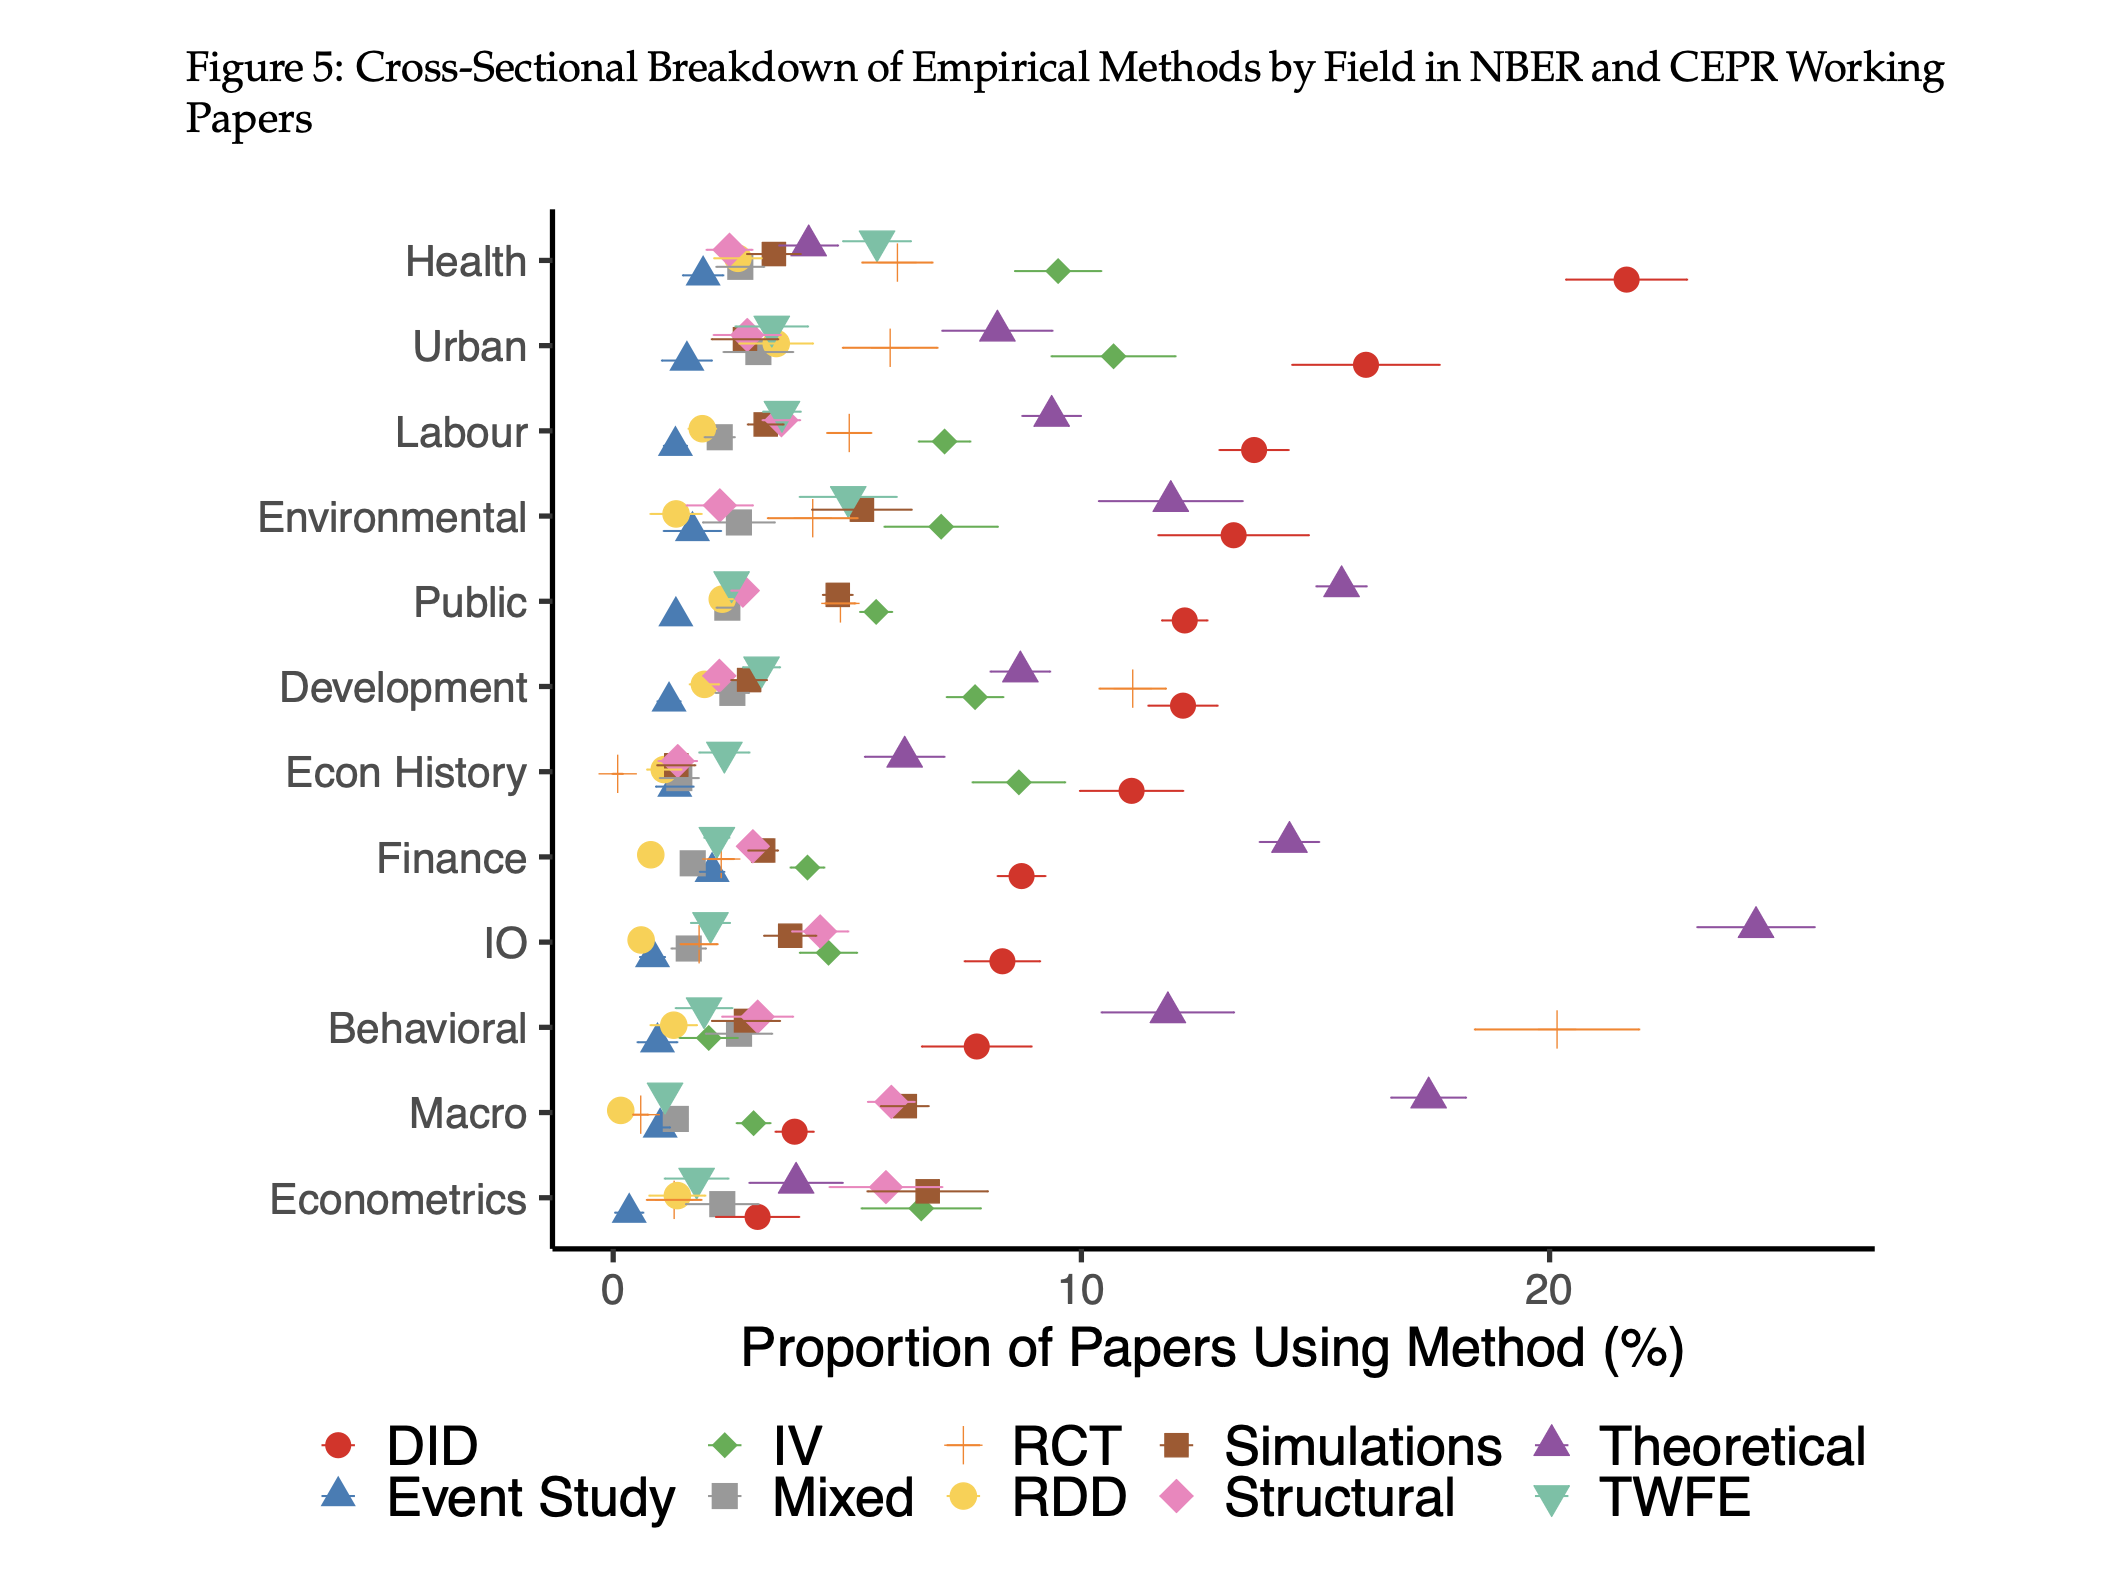
\includegraphics[width=0.7\textwidth]{../Figures/L2_did_growth2.png} \\
  \citet{garg2025causal}
\end{frame}

% -------------------------------------------------------
\begin{frame}{The 2$\times$2 setup: four averages and three subtractions}

  Two groups ($k$ = treated, $U$ = untreated), two periods (Pre, Post).

  \medskip
  \begin{center}
  \small
  \begin{tabular}{lcc|c}
    \toprule
    & Pre & Post & $\Delta$ \\
    \midrule
    Treated ($k$)   & $\bar Y_k^{pre}$ & $\bar Y_k^{post}$ & $\bar Y_k^{post} - \bar Y_k^{pre}$ \\
    Untreated ($U$) & $\bar Y_U^{pre}$ & $\bar Y_U^{post}$ & $\bar Y_U^{post} - \bar Y_U^{pre}$ \\
    \midrule
    \textbf{DD}     & & & $\hat\delta^{DD} = (\bar Y_k^{post} - \bar Y_k^{pre}) - (\bar Y_U^{post} - \bar Y_U^{pre})$ \\
    \bottomrule
  \end{tabular}
  \end{center}

  \medskip
  OLS representation:
  \[
    Y_{ist} = \alpha + \gamma \cdot \text{Treat}_s + \lambda \cdot \text{Post}_t
              + \textcolor{ecblue}{\delta} \cdot (\text{Treat}_s \times \text{Post}_t) + \varepsilon_{ist}
  \]

  \begin{itemize}
    \item $\hat\delta$ is the coefficient on the interaction term
    \item Absorbs pre-existing level differences ($\gamma$) and common time trends ($\lambda$)
  \end{itemize}

\end{frame}

% -------------------------------------------------------
\begin{frame}{Parallel trends: the identifying assumption}

  \begin{columns}[T]
    \begin{column}{0.5\textwidth}
      \textbf{Formal statement}
      \[
        E[Y_t^0 - Y_{t-1}^0 \mid D=1] = E[Y_t^0 - Y_{t-1}^0 \mid D=0]
      \]
      In the absence of treatment, treated and untreated units would have followed the \emph{same trend}.

      \bigskip
      \textbf{What it is not}
      \begin{itemize}
        \item Not ``same levels'' — DiD removes level differences
        \item Not testable in the post-period (we observe $Y^1$, not $Y^0$, for treated)
        \item Pre-trend tests are informative but \alert{not sufficient}
      \end{itemize}
    \end{column}
    \begin{column}{0.45\textwidth}
      % TikZ counterfactual diagram
      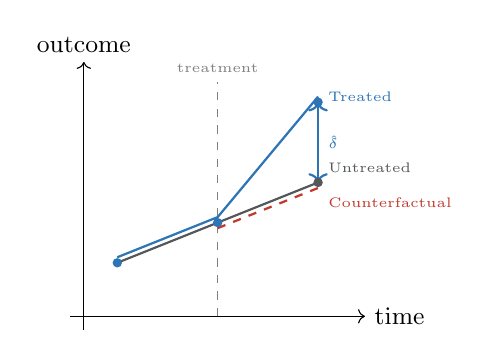
\begin{tikzpicture}[scale=0.85]
        \draw[->] (-0.2,0) -- (4.2,0) node[right]{\small time};
        \draw[->] (0,-0.2) -- (0,3.8) node[above]{\small outcome};
        % Pre period marker
        \draw[dashed, gray] (2,0) -- (2,3.5) node[above]{\tiny treatment};
        % Untreated path (reference, no shift)
        \draw[thick, ecgray] (0.5,0.8) -- (2,1.4) -- (3.5,2.0)
              node[above right]{\tiny Untreated};
        % Treated actual (shifted up 2pt — separates from untreated in pre-period)
        \draw[thick, ecblue, transform canvas={yshift=2pt}]
              (0.5,0.8) -- (2,1.4) -- (3.5,3.2)
              node[right]{\tiny Treated};
        % Counterfactual (shifted down 2pt — separates from untreated in post-period)
        \draw[thick, ecred, dashed, transform canvas={yshift=-2pt}]
              (2,1.4) -- (3.5,2.0)
              node[below right]{\tiny \color{ecred}Counterfactual};
        % ATT brace
        \draw[<->, thick, ecblue] (3.5,2.0) -- (3.5,3.2)
              node[midway, right]{\tiny $\hat\delta$};
        % Dots
        \fill[ecblue] (0.5,0.8) circle (2pt);
        \fill[ecblue] (2,1.4) circle (2pt);
        \fill[ecblue] (3.5,3.2) circle (2pt);
        \fill[ecgray] (3.5,2.0) circle (2pt);
      \end{tikzpicture}
    \end{column}
  \end{columns}

\end{frame}

% -------------------------------------------------------
\begin{frame}{Two auxiliary assumptions}

  \begin{block}{No anticipation}
    Treatment has no effect on potential outcomes before the treatment date.
    \[
      Y_{it}^1 = Y_{it}^0 \quad \forall\, t < T^*
    \]
    Violation: firms start adjusting hiring \emph{before} a policy is announced.
    Pre-treatment event-study coefficients should be zero under this assumption.
  \end{block}

  \bigskip

  \begin{block}{SUTVA (Stable Unit Treatment Value Assumption)}
    \begin{itemize}
      \item \textbf{No interference:} treatment of unit $i$ does not affect outcomes of unit $j$
      \item \textbf{No hidden versions:} there is a single version of treatment
    \end{itemize}
    Violation: a local job-training programme creates spillovers to untreated workers in the same city.
  \end{block}

\end{frame}

% -------------------------------------------------------
\begin{frame}{Falsification strategies: making the case for parallel trends}

  Three complementary tools \citep{cunningham2021}:

  \begin{enumerate}
    \item \textbf{Event-study pre-trends}: regress on leads and lags of treatment.
          Pre-treatment coefficients should be statistically indistinguishable from zero.

    \item \textbf{Same outcome, different group}: apply the same DiD to a group that
          should be unaffected. If that group also shows an effect, something is wrong.
          \emph{Example:} Medicaid expansion on the near-elderly vs.\ the elderly (already on Medicare).

    \item \textbf{Same group, placebo outcome}: apply the DiD to an outcome that the
          treatment \emph{cannot} affect.
          \emph{Example:} test whether a minimum wage affects \emph{pre-reform} employment.
  \end{enumerate}

  \begin{alertblock}{Important}
    None of these tests \emph{proves} parallel trends — they make it more or less \emph{plausible}.
    Parallel trends is a fundamentally untestable assumption about an unobserved counterfactual.
  \end{alertblock}

\end{frame}

% -------------------------------------------------------
\begin{frame}{From 2$\times$2 to panel: TWFE}

  With multiple units and periods, estimate:
  \[
    Y_{it} = \alpha_i + \gamma_t + \textcolor{ecblue}{\delta}\, D_{it} + \varepsilon_{it}
  \]
  \begin{itemize}
    \item $\alpha_i$: unit fixed effects — absorb all time-invariant heterogeneity
    \item $\gamma_t$: time fixed effects — absorb common shocks
    \item $D_{it}$: treatment indicator (switches on at treatment date)
  \end{itemize}

  \medskip
  \textbf{Why does this work? Frisch-Waugh-Lovell (FWL)}

  Absorbing $\alpha_i + \gamma_t$ by demeaning is equivalent to projecting out unit and time means.
  $\hat\delta$ is identified from \emph{within-unit, within-time-period} variation in treatment
  after removing unit trends and time shocks. This is the \textbf{two-way within-group estimator}.

  \begin{exampleblock}{When TWFE $= $ ATT}
    Under homogeneous and constant treatment effects and a single treatment cohort,
    TWFE recovers the ATT. These conditions break down with \emph{staggered adoption}.
  \end{exampleblock}

\end{frame}

% ============================================================
\section{Controls in DiD: Handle with Care}
% ============================================================

\begin{frame}{Controls in DiD are not like controls in OLS}

  \textbf{In cross-sectional OLS}: controls absorb confounders that bias the coefficient of interest.

  \medskip
  \textbf{In DiD}: the design already removes time-invariant differences. Controls serve a \emph{different} purpose:
  they help justify \textbf{conditional parallel trends} when unconditional trends differ.

  \bigskip
  \begin{alertblock}{The problem with ``just adding controls'' to TWFE \citep{huntingtonklein2023}}
    If covariates are \textbf{time-varying}, including them in TWFE can introduce new bias:
    \begin{itemize}
      \item A post-treatment covariate that is itself affected by treatment is a \emph{bad control}
      \item Pre-treatment covariate levels are safe; their post-treatment realisations are not
      \item Matching on pre-treatment values (or interacting covariates with time) is the correct approach
    \end{itemize}
  \end{alertblock}

  \medskip
  \textbf{Safe strategies}: include only \emph{pre-treatment} covariate values; use propensity-score weighting;
  or use the doubly-robust CS estimator which handles covariates correctly by design.

\end{frame}

% ============================================================
\section{TWFE with Staggered Adoption: What Goes Wrong}
% ============================================================

\begin{frame}{Staggered adoption: the real-world setting}

  In practice, units often adopt treatment at \emph{different times}:
  \begin{itemize}
    \item US states adopt right-to-carry laws in different years
    \item Firms undergo M\&A in different waves
    \item Italian departments receive the Excellence award in a single cohort (2018) — but evaluated vs.\ control departments at different distances in calendar time
  \end{itemize}

  \medskip
  With staggered timing and multiple cohorts, TWFE still runs fine — but what does $\hat\delta$ identify?

  \begin{alertblock}{The Bacon (2021) insight}
    TWFE with staggered adoption is a \textbf{variance-weighted average of all possible $2\times 2$ DiDs} —
    including comparisons that use \emph{already-treated} units as controls.
    These ``forbidden comparisons'' can produce negative weights and contaminate the estimate.
  \end{alertblock}

\end{frame}

% -------------------------------------------------------
\begin{frame}{The Bacon decomposition}

  With treatment groups $k$ (early) and $l$ (late) plus never-treated $U$, TWFE decomposes as:
  \[
    \hat\delta^{\,TWFE} = \sum_{k \neq U} s_{kU}\,\hat\delta_{kU}^{2\times2}
    + \sum_{k \neq U}\sum_{l > k} s_{kl}
      \Big[\mu_{kl}\,\hat\delta_{kl}^{2\times2,k} + (1-\mu_{kl})\,\hat\delta_{lk}^{2\times2,l}\Big]
  \]

  \begin{itemize}
    \item $\hat\delta_{kU}^{2\times2}$: clean — early vs.\ never-treated (safe comparison)
    \item $\hat\delta_{kl}^{2\times2,k}$: clean — early vs.\ not-yet-treated late group (safe)
    \item $\hat\delta_{lk}^{2\times2,l}$: \alert{dangerous} — late group vs.\ \emph{already-treated} early group
  \end{itemize}

  The dangerous term picks up:
  \[
    \hat\delta_{lk}^{2\times2,l} = ATT_{l,Post(l)} + \underbrace{\Delta Y^0_l - \Delta Y^0_k}_{\text{PT bias}}
    - \underbrace{(ATT_k^{Post} - ATT_k^{Mid})}_{\text{Heterogeneity bias}}
  \]
  If treatment effects \emph{grow over time} ($ATT_k^{Post} > ATT_k^{Mid}$), the heterogeneity bias is \alert{negative},
  and TWFE can \alert{flip sign}.

\end{frame}

% -------------------------------------------------------
\begin{frame}{Baker (2022) simulation: sign flip from TWFE}

  \textbf{Design:} 1000 firms, 4 staggered cohorts, 30 years. True average ATT $= +82$. Dynamic treatment effects (effects grow over time).

  \medskip
  \begin{center}
  \small
  \begin{tabular}{lcc}
    \toprule
    Estimator & $\hat{ATT}$ & Status \\
    \midrule
    True (weighted avg.) & $+82$ & benchmark \\
    TWFE & $-6.69^{***}$ & \textcolor{ecred}{sign flipped} \\
    Callaway \& Sant'Anna & $+68.3^{***}$ & close to truth \\
    Sun \& Abraham & $+68.3^{***}$ & close to truth \\
    \bottomrule
  \end{tabular}
  \end{center}

  \medskip
  \begin{columns}[T]
    \begin{column}{0.48\textwidth}
      \textbf{Bacon decomposition of $\hat\delta^{TWFE} = -6.69$:}\\[4pt]
      \small
      \begin{tabular}{lcc}
        \toprule
        Comparison & Weight & Avg.\ DD \\
        \midrule
        Early vs.\ late (clean) & 0.50 & $+51.8$ \\
        Late vs.\ early (dirty) & 0.50 & $-65.2$ \\
        \midrule
        \multicolumn{2}{l}{Weighted sum} & $-6.69$ \\
        \bottomrule
      \end{tabular}
    \end{column}
    \begin{column}{0.45\textwidth}
      \begin{alertblock}{Key lesson}
        The sign flip is not a data problem — it is an \emph{estimator} problem.
        TWFE assigns 50\% weight to a contaminated comparison.
        Modern estimators fix this by construction.
      \end{alertblock}
    \end{column}
  \end{columns}

\end{frame}

% ============================================================
\section{Modern DiD Estimators}
% ============================================================

\begin{frame}{The forward-engineering response}

  The Bacon decomposition \emph{diagnoses} the problem but does not solve it.
  A new generation of estimators avoids the forbidden comparisons by design \citep{roth2023what}.

  \medskip
  \begin{center}
  \small
  \renewcommand{\arraystretch}{1.3}
  \begin{tabular}{p{3.5cm} p{3.5cm} p{3.5cm}}
    \toprule
    \textbf{Callaway \& Sant'Anna (2021)} & \textbf{Sun \& Abraham (2021)} & \textbf{de Chaisemartin \& D'Haultf\oe{}uille (2020)} \\
    \midrule
    Group-time ATT(g,t); aggregates via user-chosen weights &
    Interaction-weighted estimator; cohort-specific coefficients &
    ``Switchers'' approach; works with multi-valued and reversible treatment \\
    \midrule
    Never- or not-yet-treated comparison; doubly robust &
    Last-cohort or never-treated comparison &
    Comparison across switchers and non-switchers \\
    \midrule
    \texttt{csdid} (Stata) &
    \texttt{eventstudyinteract} (Stata) &
    \texttt{did\_multiplegt\_dyn} (Stata) \\
    \bottomrule
  \end{tabular}
  \end{center}

\end{frame}

% -------------------------------------------------------
\begin{frame}{Callaway \& Sant'Anna (2021): group-time ATTs}

  \textbf{Key idea:} Instead of one aggregate $\delta$, estimate a matrix of \emph{group-time ATTs}:
  \[
    ATT(g,t) = E\bigl[Y_t^1 - Y_t^0 \mid G_g = 1\bigr]
  \]
  where $G_g = 1$ identifies units first treated at time $g$.

  \medskip
  \textbf{Assumptions:}
  \begin{enumerate}
    \item Irreversible treatment (absorbing state)
    \item Conditional parallel trends (given $X$) relative to either never-treated \emph{or} not-yet-treated
    \item No anticipation
    \item Common support for the propensity score
  \end{enumerate}

  \medskip
  \textbf{Aggregation choices} — all are averages of ATT(g,t) with different weights:
  \begin{itemize}
    \item \textbf{Simple} (uniform): one overall ATT
    \item \textbf{Event-time}: ATT at each period relative to treatment ($\ell = t - g$) — the event-study plot
    \item \textbf{Calendar}: ATT by calendar year
    \item \textbf{Group}: ATT by cohort
  \end{itemize}

\end{frame}

% -------------------------------------------------------
\begin{frame}{Sun \& Abraham (2021): interaction-weighted estimator}

  \textbf{Key idea:} Augment TWFE by interacting treatment dummies with cohort indicators.
  This saturates the model and recovers cohort-specific event-study coefficients.

  \medskip
  Model:
  \[
    Y_{it} = \alpha_i + \gamma_t + \sum_{g}\sum_{\ell \neq -1}
             \delta_{g,\ell}\,\bigl(\mathbf{1}[G_i = g] \times D_{it}^{\ell}\bigr) + \varepsilon_{it}
  \]
  where $D_{it}^\ell = \mathbf{1}[t - G_i = \ell]$ is the relative-time indicator.

  \medskip
  \textbf{Aggregation:} average $\hat\delta_{g,\ell}$ across cohorts, weighting by cohort size.
  The resulting event-study plot is free of contamination from other cohorts' treatment effects.

  \begin{exampleblock}{Comparison with CS}
    SA and CS produce numerically very similar event-study plots when using the same comparison group.
    SA is more natural when you want the TWFE regression as the starting point;
    CS is more flexible (doubly robust, can use not-yet-treated).
  \end{exampleblock}

\end{frame}

% -------------------------------------------------------
\begin{frame}{de Chaisemartin \& D'Haultf\oe{}uille (2020): brief overview}

  \textbf{Setting:} treatment can be multi-valued \emph{and} reversible — more general than CS/SA.

  \medskip
  \textbf{Key idea:} focus on ``switchers'' — units whose treatment \emph{changes} between consecutive periods.
  Compare the outcome change of switchers to the outcome change of non-switchers in the same period.

  \medskip
  \textbf{Identifying assumption:} in the absence of the treatment change, switchers and non-switchers
  would have had parallel trends in that period pair.

  \medskip
  \begin{columns}[T]
    \begin{column}{0.45\textwidth}
      \textbf{When to use dCdH}
      \begin{itemize}
        \item Treatment can turn off (job loss, de-regulation)
        \item Continuous or ordinal treatment intensity
        \item You want period-by-period robust estimates
      \end{itemize}
    \end{column}
    \begin{column}{0.45\textwidth}
      \textbf{When to use CS/SA instead}
      \begin{itemize}
        \item Binary absorbing treatment
        \item You want cohort-level heterogeneity
        \item Long panels with many pre-periods
      \end{itemize}
    \end{column}
  \end{columns}

\end{frame}

% -------------------------------------------------------
\begin{frame}{Clustering and inference in DiD}

  \begin{block}{At what level should you cluster?}
    Cluster at the level at which treatment is assigned — \emph{not} at the observation level.
    \begin{itemize}
      \item Policy varies at state level $\rightarrow$ cluster by state
      \item M\&A event varies by firm $\rightarrow$ cluster by firm
      \item DoE treatment varies by department $\rightarrow$ cluster by department
    \end{itemize}
  \end{block}

  \begin{alertblock}{The few-clusters problem}
    Standard cluster-robust SEs require many clusters (rule of thumb: $\geq 30$--50).
    With few treated clusters, SEs are downward biased and rejection rates inflated.\\[4pt]
    \textbf{Solutions:} wild cluster bootstrap (\texttt{boottest}); randomisation inference;
    or report both cluster-robust and wild-bootstrap CIs.
  \end{alertblock}

  \medskip
  The CS and SA estimators use the \emph{influence function} approach for SEs —
  robust to heteroskedasticity and correctly accounts for estimation of the propensity score.

\end{frame}

% ============================================================
\section{Sensitivity Analysis: HonestDiD}
% ============================================================

\begin{frame}{The pre-trends test is not enough}

  Event-study pre-treatment coefficients being ``flat'' is reassuring but \alert{insufficient} \citep{roth2022pretest}.

  \medskip
  \textbf{Three fundamental limitations:}

  \begin{enumerate}
    \item \textbf{Parallel pre-trends $\neq$ parallel counterfactual post-trends.}
          A simultaneous policy change in the post-period could create parallel pre-trends
          but non-parallel post-trends.

    \item \textbf{Low power.}
          Pre-trend tests are typically underpowered. We can fail to detect economically meaningful
          pre-trends. Roth (2022): in papers from \textit{AER}, \textit{AEJ Applied}, \textit{AEJ Policy},
          the pre-trend test had only 50--80\% power against violations that would substantially bias the estimate.

    \item \textbf{Pre-testing distortions.}
          Conditioning on a non-significant pre-trend introduces a form of \emph{selection bias}:
          we are analysing a selected subsample of draws where the noise happened to look flat,
          which inflates the post-treatment estimate.
  \end{enumerate}

\end{frame}

% -------------------------------------------------------
\begin{frame}{Rambachan \& Roth (2023): a more credible approach}

  \textbf{Core idea:} Rather than testing whether trends are exactly parallel, impose
  \emph{restrictions on how far they can deviate}.

  \medskip
  Let $\delta_t$ denote the violation of parallel trends in period $t$:
  \[
    \delta_t = E[Y_t^0 - Y_{t-1}^0 \mid D=1] - E[Y_t^0 - Y_{t-1}^0 \mid D=0]
  \]
  We observe $\hat\delta_{pre}$ (pre-treatment trend). We do not observe $\delta_{post}$.

  \medskip
  \textbf{Restriction options:}
  \begin{itemize}
    \item \textbf{Smoothness (M):} the post-trend cannot deviate more than $M$ from a linear
          extrapolation of the pre-trend
          \[ |\delta_{post} - \text{linear extrapolation of }\hat\delta_{pre}| \leq M \]
    \item \textbf{Relative magnitudes ($\bar M$):} $|\delta_{post}| \leq \bar M\,|\delta_{pre}|$
  \end{itemize}

  For each value of $M$, compute a \emph{robust confidence interval}.
  Report how the CI changes as $M$ grows — the \textbf{sensitivity plot}.

\end{frame}

% -------------------------------------------------------
\begin{frame}[shrink=8]{How to read a HonestDiD sensitivity plot}

  \begin{columns}[T]
    \begin{column}{0.48\textwidth}
      \textbf{Axes:}
      \begin{itemize}
        \item $x$-axis: $M$ — the amount of allowed trend deviation
        \item $y$-axis: the robust 95\% confidence interval for the ATT
      \end{itemize}

      \bigskip
      \textbf{Reading the plot:}
      \begin{itemize}
        \item At $M=0$: standard CI (assumes exact parallel trends)
        \item As $M$ grows: CI widens — we allow more deviation
        \item Find the \emph{breakdown $M$}: the value at which the CI crosses zero
        \item Ask: is that level of trend deviation \emph{plausible} given the pre-trend?
      \end{itemize}

      \bigskip
      \begin{exampleblock}{Practical benchmark}
        A common choice: $M$ equal to the largest estimated pre-trend coefficient.
        This asks: ``What if the post-period trend deviates as much as the worst pre-period trend?''
      \end{exampleblock}
    \end{column}
    \begin{column}{0.48\textwidth}
      % TikZ schematic sensitivity plot
      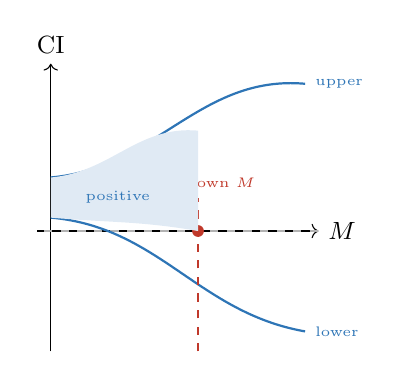
\begin{tikzpicture}[scale=0.85]
        \draw[->] (-0.2,0) -- (4.0,0) node[right]{\small $M$};
        \draw[->] (0,-1.8) -- (0,2.5) node[above]{\small CI};
        % zero line
        \draw[dashed, gray!60] (-0.1,0) -- (4.0,0);
        % upper bound (widening)
        \draw[thick, ecblue] (0,0.8) to[out=5, in=175] (3.8,2.2)
              node[right]{\tiny upper};
        % lower bound (crossing zero)
        \draw[thick, ecblue] (0,0.2) to[out=-5, in=170] (3.8,-1.5)
              node[right]{\tiny lower};
        % breakdown point
        \draw[dashed, ecred] (2.2,-1.8) -- (2.2,0.5)
              node[above]{\tiny \color{ecred} breakdown $M$};
        \fill[ecred] (2.2,0) circle (2.5pt);
        % shaded region for positive CI
        \fill[ecblue!15] (0,0.2) -- (0,0.8)
              to[out=5, in=175] (2.2,1.5)
              -- (2.2,0) to[out=170, in=-5] (0,0.2);
        \node at (1.0, 0.5) {\tiny \color{ecblue} positive};
      \end{tikzpicture}
    \end{column}
  \end{columns}

\end{frame}

% ============================================================
\section{Lab Preview}
% ============================================================

\begin{frame}[shrink=5]{Lab 2: two applied examples}

  \begin{columns}[T]
    \begin{column}{0.48\textwidth}
      \begin{block}{Exercise 1 — Departments of Excellence}
        \textbf{Question:} Did the Italian Academic Excellence Initiative
        (2018--) raise faculty recruitment in awarded departments?

        \medskip
        \textbf{Data:} 290 university departments, balanced panel 2013--2020.
        Single treatment cohort (2018). Source: \citet{rizzo2025doe}.

        \medskip
        \textbf{Methods:}
        \begin{itemize}\small
          \item Descriptives + raw trends
          \item TWFE static \& event study
          \item Conditional parallel trends test
          \item Callaway \& Sant'Anna (\texttt{csdid})
          \item HonestDiD sensitivity plot
        \end{itemize}
      \end{block}
    \end{column}
    \begin{column}{0.48\textwidth}
      \begin{block}{Exercise 2 — Superstar M\&A}
        \textbf{Question:} Do technology-related M\&As raise acquirer markups?

        \medskip
        \textbf{Data:} Firm-level panel, staggered by M\&A year.
        Source: \citet{rentocchini2025superstar}.

        \medskip
        \textbf{Methods:}
        \begin{itemize}\small
          \item TWFE static \& event study
          \item Bacon decomposition (\texttt{bacondecomp})
          \item CS \& SA combined event-study plot
          \item HonestDiD sensitivity plot
        \end{itemize}
      \end{block}
    \end{column}
  \end{columns}

  \bigskip
  \begin{center}
    \textbf{Script:} \texttt{Lab/L2\_did.do}
  \end{center}

\end{frame}

% ============================================================
% References
% ============================================================

\begin{frame}[allowframebreaks]{References}
  \small
  \bibliography{../Bibliography_base}
\end{frame}

\end{document}
